\section{Playing with survival rates}
Exponential discounting comes from perhaps the simplest model imaginable. A squirel should be indifferent
between two findings whenever they are equal in expected value. If a squirrel has geometric survival (with parameter
$s$), then a future payment $F_t$ (at time $t$) is, in expectation, $s^t F_t$. I now ask: what survival rates give
hyperbolic discounting? 
\begin{itemize}
    \item At $t = 1$, we require $\frac{1}{1 + h} = s_0$. Rearranging gives $h = \frac{1 - s_0}{s_0}$. 
    \item By induction we can show that $s_0\cdot s_1 \cdot \ldots \cdot s_t = \frac{1}{1 + ht}$ whenever
        $s_a = \frac{ (a - 1) - (a - 2)s_0}{a - (a - 1)s_0}$. 
\end{itemize}
For instance, if initial survival is $s_0 = 1/2$, then survival must grow according to $s_a = \frac{a+1}{a+2} = \frac{2}{3}, \frac{3}{4}, 
\frac{4}{5},\ldots$ in order for a squirrel to discount hyperbolically in the simplistic model wherein a future payment is equal to
its expected value.

\subsection{Age structured model}
Fix squirrels with  birth and survival distributions $b_0, \ldots, b_A$ and $s_0, \ldots, s_{A-1}$, leading to a Lyapunov exponent
of $\lambda_0 = \lambda(b, s)$. The experimental approach of offering a payment of $P$ immediately and increasing/decreasing future payments $F_t$ until
indifference can be closely approximated.
\begin{enumerate}
    \item Increase initial fecundity $b_0$ to $b_0 + P$. 
    \item Compute $\lambda' = \lambda(b_0 + P, \text{ all else same }) $. 
    \item Determine $F_1$ such that $\lambda(b_0, b_1 + F_a, b_2, \ldots) = \lambda'$. Interpretation: a squirrel is fitness
        indifferent between a payment of $P$ at age $0$ and $F_1$ at age $1$.
    \item Repeat for $a = 2, \ldots, A$. 
    \item The resulting list $\left[ P, F_1, F_2, \ldots, F_A \right]$ tracks the required appreciation of $P$ for indifference.
\end{enumerate}
The expected payout model predicts that appropriately increasing survival should lead to hyperbolic discounting \textit{
independent of fecundity}. How does this hold up in practice?
Take $A = 10$, and $s = [1/2, 2/3, 3/4, 4/5, 5/6, 6/7, 7/8, 8/9, 9/10, 10/11]$. For simplicity, the birth vector
will be $\left[ b, b, b, \ldots, b \right]$. The population has age independent fecundity. We vary $b$ in order to understand
the appreciation trend of an initial payment of $0.01$. We find that the most important difference is whether $\lambda_0 \lessgtr  1$. 
\begin{figure}[H]
    \centering
    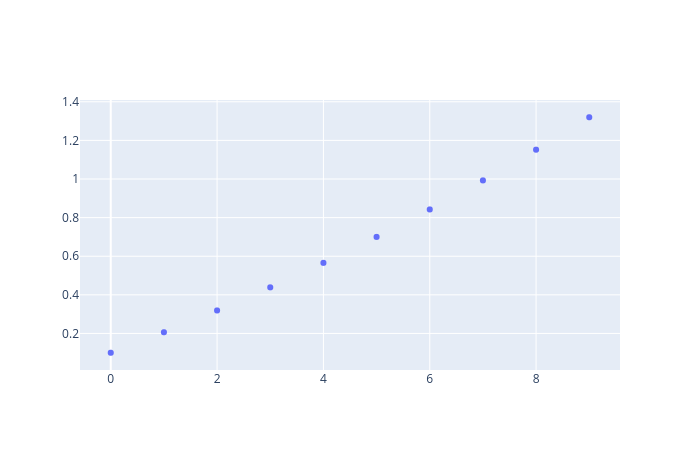
\includegraphics[scale = 0.7]{reqd_fec_increase_unit_fitness.png}
    \caption{Appreciation of 0.1 for a life history with $\lambda_0 = 1$.}
\end{figure}
\begin{figure}[H]
    \centering
    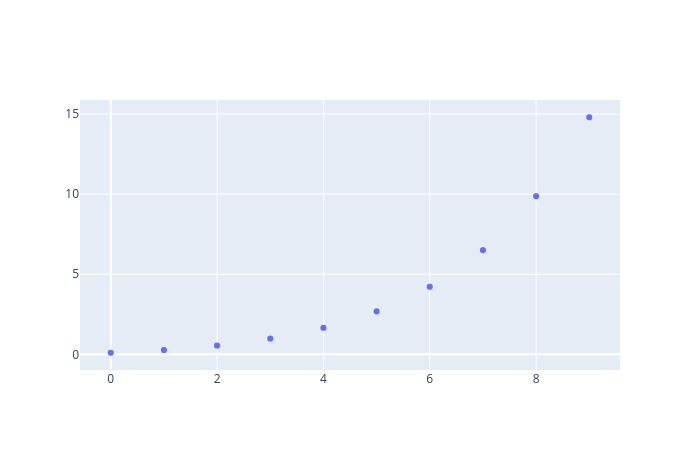
\includegraphics[scale = 0.7]{reqd_fec_increase_fitness_ge1.png}
    \caption{Appreciation of 0.1 for a life history with $\lambda_0 = 1.3 > 1$.}
\end{figure}
\begin{figure}[H]
    \centering
    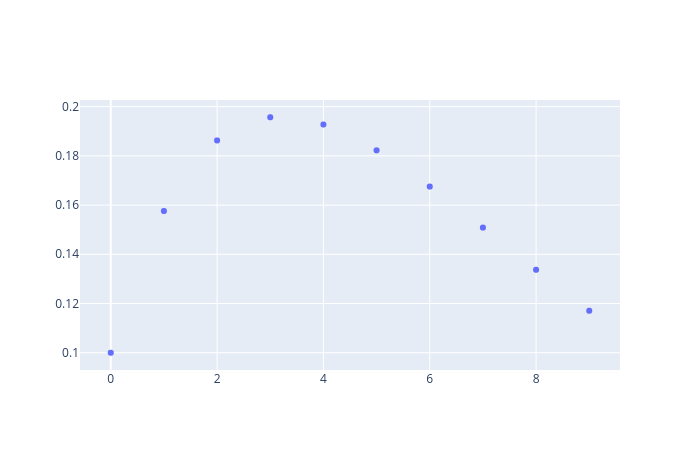
\includegraphics[scale = 0.7]{reqd_fec_increase_fitness_le1.png}
    \caption{Appreciation of 0.1 for a life history with $\lambda_0 = 0.75 < 1$.}
\end{figure}
This seems fantastic. Can I give some kind of analytic rationale for why such richness in discounting schemes? It runs out we have
done enough work already to understand. Remember that 
$$ \frac{\d \lambda}{\d b_{\alpha}} \approx \lambda^{-\alpha}\cdot \left( s_0\cdot\ldots\cdot s_{\alpha - 1} \right)$$
where $\approx$ is taken to mean both approximately equal and proportional to (proportionality doesn't matter - we can scale a discounting
function by any constant, since only relative size matters). If $\lambda = 1$, we get exactly the simplistic expected payment model.
If $\lambda > 1$, we have a product of exponential and hyperbolic discounting, and the exponential term will tend to dominate. Finally,
if $\lambda < 1$, we have negative exponential discounting at the same time as hyperbolic discounting. The exponential term will tend to
value \textit{future payments more heavily than present value}, explaining the $\cap$ shape we see in the third figure. 
Our analysis is really only valid for marginal increases in $b_0$. Too large an increase will push $\lambda \gg 1$, and the exponential
term will again dominate.
\begin{figure}[H]
    \centering
    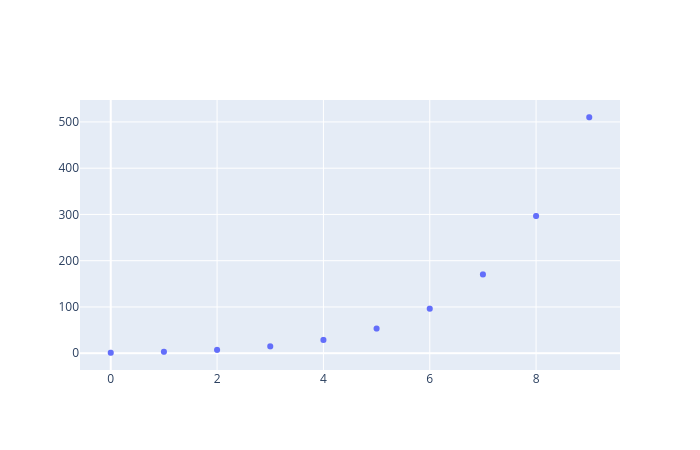
\includegraphics[scale = 0.7]{reqd_fec_increase_bigP.png}
    \caption{Appreciation of 1 for a life history with $\lambda_0 = 1$.}
\end{figure}
We can get creative, however, and vary $\lambda$ to compensate for a big $P$ so as to still come away with hyperbolic discounting. 
 \begin{figure}[H]
    \centering
    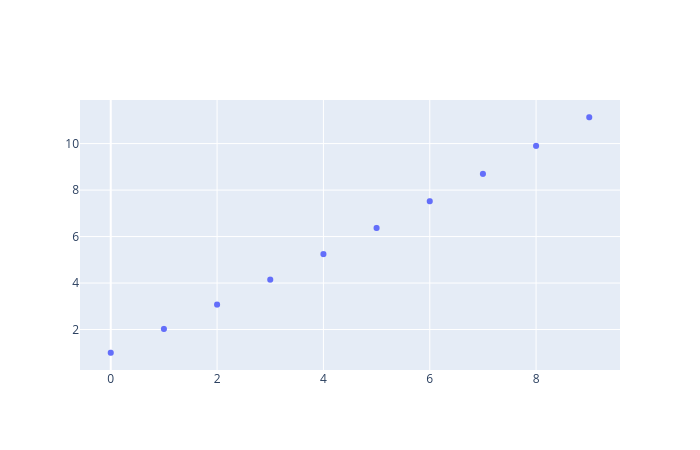
\includegraphics[scale = 0.7]{reqd_fec_increase_bigP_low_fitness.png}
    \caption{Appreciation of 1 for a life history with $\lambda_0 = 0.5$.}
\end{figure}  
\subsection{A conspiracy theory}
It took me a while to remember from where I recognized the sequence $\frac{1}{2}, \frac{2}{3}, \frac{3}{4}, \ldots$. Do you remember?
It actually came about earlier in this document, when discussing increasing survival as a squirrel's cache of nuts increases. 
Briefly, two nuts were found daily, and a squirrel has survival $s_{\beta}$ when it has $\beta$ nuts saved. A question I asked at 
the time was: For what values of $s_0, s_1, \ldots, s_{\hat \beta}$ does a squirrel have unit fitness? It turns out that
the same pattern as leads to hyperbolic discounting leads to unit survival in the increasing survival with banked nuts model. 
At a high level:
\begin{enumerate}
    \item Looking for unit fitness $\Rightarrow$ $s = \frac{1}{2}, \frac{2}{3}, \frac{3}{4}, \ldots$
    \item Looking for hyperbolic discount $\Rightarrow$ $s = \frac{1}{2}, \frac{2}{3}, \frac{3}{4}, \ldots$
\end{enumerate}
We have what seems to be an awfully big coincidence here. To quote Jaye, who was quoting someone else, ``correlation does not
imply causation, but it does imply unresolved causal structure.'' I want to find that structure! Is it possible that unit
fitness and hyperbolic discounting go hand in hand? I can rule that out: if $s_a$ is constant and $b$ is such that $\lambda = 1$,
then we will still have exponential discounting. I'm rambling, but this is interesting to think about.




